\chapter{Metodologia}\label{cap:metodologia}

Este capítulo descreve o projeto do gerador. Primeiro, apresenta a visão geral do sistema, suas especificações e a versão anterior do gerador, que serviu de ponto de partida; em seguida, o projeto do núcleo digital, do controle pelo computador, da verificação por simulação, da interface com o usuário e da placa analógica. Todos os arquivos do projeto (código \ac{vhdl}, \eng{testbenches}, interface, projeto da placa e simulações) estão disponíveis no repositório do trabalho \cite{seifert2026}; a organização do repositório é descrita no Apêndice~\ref{ap:repositorio}. Os instrumentos e os programas usados estão nos Apêndices~\ref{ap:instrumentos} e~\ref{ap:softwares}.

\section{Visão geral do sistema}

O sistema tem três partes, mostradas na Figura~\ref{fig:sistema}. No computador, uma interface gráfica em Python envia os comandos através do programa \cod{quartus\_stp} e do USB-Blaster da DE2-115. No \ac{fpga}, o bloco de controle recebe os comandos pelo Virtual \ac{jtag} e configura o núcleo \ac{dds}, que entrega uma amostra de 8~bits a cada ciclo do clock de 10~MHz, gerado por um \ac{pll} a partir do oscilador de 50~MHz da placa. As amostras saem pelo conector de expansão da placa para a placa analógica, onde o DAC0800 as converte em corrente e os amplificadores operacionais as convertem em tensão, filtram e ajustam a amplitude.

\begin{figure}
	\caption{Diagrama de blocos do sistema.}
	\label{fig:sistema}
	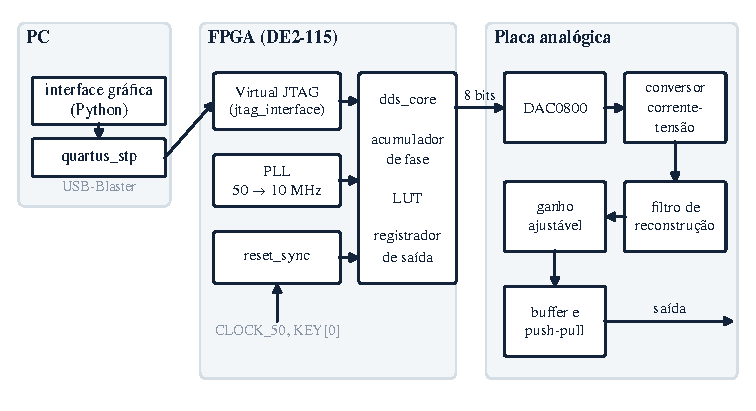
\includegraphics[width=\textwidth]{./figuras/sistema}
	\legend{Fonte~---~Autoria própria.}
\end{figure}

\section{Especificações}

A Tabela~\ref{tab:especificacoes} reúne os parâmetros do gerador. A frequência de clock de 10~MHz foi escolhida pelo tempo de acomodação típico do DAC0800, de 100~ns \cite{ti2013}: com um clock mais rápido, as amostras mudariam antes de o conversor se acomodar. O acumulador de 32~bits dá a resolução de 2,33~mHz da Equação~(\ref{eq:resolucao}). A tabela de 1024~amostras (\(P = 10\)) limita os espúrios de truncamento a cerca de \(-60\)~dBc, valor próximo ao limite de cerca de 50~dB imposto pela quantização em 8~bits, conforme as Equações~(\ref{eq:snr}) e (\ref{eq:sfdr}).

A frequência é pedida pelo computador como um inteiro em hertz, de 18~bits, que é a largura do registrador de dados do protocolo (Seção~\ref{sec:controle}). A frequência máxima, de 262\,143~Hz, fica muito abaixo do limite de Nyquist de 5~MHz e garante pelo menos 38 amostras por período.

\begin{table}
	\caption{Especificações do gerador.}
	\label{tab:especificacoes}
	\begin{tabular}{l l}\toprule
		Parâmetro & Valor\\\midrule
		Clock do \ac{dds} (\(f_{clk}\)) & 10~MHz, gerado por \ac{pll} a partir de 50~MHz\\
		Acumulador de fase (\(N\)) & 32~bits\\
		Resolução de frequência (\(\Delta f\)) & 2,33~mHz\\
		Endereço da tabela (\(P\)) & 10~bits (1024 amostras por período)\\
		Amostra e \ac{dac} (\(D\)) & 8~bits, binário deslocado (zero em 128)\\
		Faixa de frequência & 0 a 262\,143~Hz, inteiro em hertz\\
		Formas de onda & seno, rampa, sinc e arbitrária\\
		Forma inicial da tabela arbitrária & eletrocardiograma sintético\\
		Configuração após o \eng{reset} & seno de 1~kHz\\
		Controle & computador, via Virtual \ac{jtag} e USB-Blaster\\\bottomrule
	\end{tabular}
	\legend{Fonte~---~Autoria própria.}
\end{table}

\section{Ponto de partida: o código legado}\label{sec:legado}

O projeto partiu de uma versão anterior do gerador, usada em bancada até setembro de 2026 e guardada no repositório em \cod{fpga/legado/}. Essa versão segue a arquitetura clássica da Figura~\ref{fig:dds_blocos}: um acumulador de fase de 32~bits e uma tabela de seno de 256 posições de 8~bits, endereçada pelos 8~bits mais significativos da fase. Todo o circuito roda no oscilador de 50~MHz da placa. Um contador gera um pulso de habilitação a cada 50 ciclos, de modo que o acumulador avança e o \ac{dac} recebe uma amostra nova a 1~MHz. A palavra de sintonia vem de cinco constantes calculadas à mão e escolhidas pelas chaves SW0 a SW4 da placa: 100~Hz, 1~kHz, 10~kHz, 100~kHz e 300~kHz. A amostra passa por um registrador antes dos pinos, e o pino 2 do conector de expansão leva um clock de 1~MHz para um \ac{dac} com registrador de entrada.

Essa versão comprovou a cadeia completa, do \ac{fpga} à placa analógica, mas suas limitações orientaram o projeto final (Tabela~\ref{tab:legado}). Ela só gerava senos, em cinco frequências fixas, e qualquer outra frequência exigia recalcular a constante e recompilar o projeto. Com a taxa de 1~MHz, a 300~kHz restavam pouco mais de três amostras por período, e a tabela de 256 posições limita o maior espúrio de truncamento de fase a cerca de \(-48\)~dBc, pela Equação~(\ref{eq:sfdr}). O código tinha três entidades, com o divisor, a seleção de frequência e o registrador de saída reunidos no topo, e foi verificado apenas por inspeção visual das formas de onda no simulador. Do código legado, o projeto final manteve a pinagem do \ac{dac}, para que a placa analógica e o cabo continuassem os mesmos, e o registrador de saída.

\begin{table}
	\caption{Comparação entre o código legado e o projeto final.}
	\label{tab:legado}
	\begin{tabular}{p{0.2\textwidth} p{0.36\textwidth} p{0.36\textwidth}}\toprule
		& Código legado & Projeto final\\\midrule
		Taxa de amostras & 1~MHz, habilitação a cada 50 ciclos de 50~MHz & 10~MHz, gerada por um \ac{pll}\\
		Tabelas & seno, \(256 \times 8\)~bits & seno, rampa, sinc e arbitrária regravável, \(1024 \times 8\)~bits\\
		Frequência & cinco valores fixos, de 100~Hz a 300~kHz & qualquer inteiro de 0 a 262\,143~Hz\\
		Palavra de sintonia & constantes calculadas à mão & multiplicação em ponto fixo no \ac{fpga}\\
		Controle & chaves da placa & computador, pelo Virtual \ac{jtag}\\
		Organização & três entidades & uma entidade por função\\
		Verificação & inspeção visual no simulador & 16 \eng{testbenches} auto-verificáveis\\
		Recursos & 72 elementos lógicos e 2\,048 bits de memória & 378 elementos lógicos e 32\,768 bits de memória\\\bottomrule
	\end{tabular}
	\legend{Fonte~---~Autoria própria.}
\end{table}

\section{Projeto do núcleo digital}

\subsection{Organização hierárquica}

O projeto digital foi organizado em blocos encapsulados: cada função fica em uma entidade \ac{vhdl} própria, com portas bem definidas, e as entidades de nível mais alto apenas instanciam e ligam as de nível mais baixo. A entidade do topo, \cod{DDS}, não contém lógica: liga o \ac{pll}, o sincronizador de \eng{reset}, o controle pelo computador, o núcleo \ac{dds} e a saída de clock do \ac{dac} aos pinos da placa. A Figura~\ref{fig:hierarquia} mostra a hierarquia completa.

As constantes compartilhadas, como as larguras do caminho de dados, os códigos das instruções do protocolo e os códigos das formas de onda, ficam em um único pacote, \cod{dds\_pkg}. Assim, cada valor é definido em um único lugar, e os blocos e os \eng{testbenches} usam as mesmas definições.

\begin{figure}
	\caption{Hierarquia das entidades \acs{vhdl} do projeto. Os blocos em cinza são \acsp{ip} gerados pelas ferramentas da Intel.}
	\label{fig:hierarquia}
	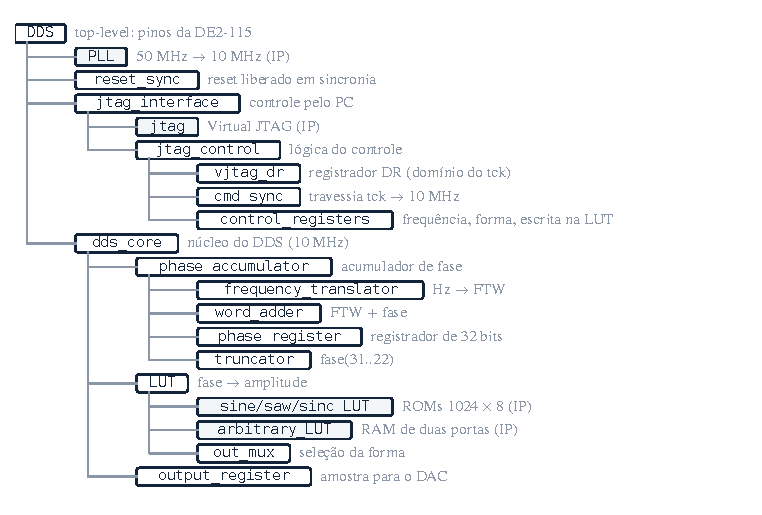
\includegraphics[width=\textwidth]{./figuras/hierarquia}
	\legend{Fonte~---~Autoria própria.}
\end{figure}

\subsection{Acumulador de fase e conversão de frequência}

O acumulador de fase (\cod{phase\_accumulator}) é composto por quatro blocos: o conversor de frequência (\cod{frequency\_translator}), o somador de 32~bits (\cod{word\_adder}), o registrador de fase (\cod{phase\_register}), que atualiza na borda de subida do clock e tem \eng{reset} assíncrono, e o truncador (\cod{truncator}), que entrega os 10~bits mais significativos da fase como endereço da tabela.

Pela Equação~(\ref{eq:fout}), a palavra de sintonia para uma frequência \(f\) é \(M = f \cdot 2^{32}/f_{clk}\), o que exigiria uma divisão. Como \(f_{clk}\) é fixo, a divisão foi substituída por uma multiplicação por uma constante em ponto fixo, com 24~bits fracionários:
\begin{equation}\label{eq:ftw}
	K = \operatorname{round}\!\left(\frac{2^{56}}{f_{clk}}\right) = 7\,205\,759\,404, \qquad M = \left\lfloor \frac{f \cdot K}{2^{24}} \right\rfloor.
\end{equation}
O produto de \(f\) (18~bits) por \(K\) (33~bits) tem 51~bits, e o deslocamento de 24~bits para a direita é apenas a escolha dos fios de saída. Como \(K\) é ligeiramente maior que o valor exato, o erro de \(M\) fica abaixo de 1~\ac{lsb} para toda a faixa de entrada, o que corresponde a um erro de frequência menor que \(\Delta f\). Na síntese, a multiplicação ocupa quatro multiplicadores de \(9 \times 9\)~bits do \ac{fpga}.

\subsection{Tabelas de forma de onda}

A conversão de fase em amplitude (\cod{LUT}) reúne quatro memórias de \(1024 \times 8\)~bits, implementadas pelo \ac{ip} \cod{altsyncram} nos blocos M9K, e um multiplexador (\cod{out\_mux}) controlado pelo sinal \cod{sel}. Três delas são \acp{rom} inicializadas por arquivos \ac{mif}, gerados conforme a Equação~(\ref{eq:lut_seno}):
\begin{itemize}
	\item seno (\cod{sel} = \cod{00}): \(\operatorname{round}(128 + 127\sin(2\pi n/1024))\);
	\item rampa (\cod{sel} = \cod{01}): subida e descida linear, em fase com o seno;
	\item sinc (\cod{sel} = \cod{10}): \(\operatorname{round}(128 + 127\,\mathrm{sinc}((n-512)/64))\), com o argumento entre \(-8\) e 8.
\end{itemize}

A quarta memória (\cod{sel} = \cod{11}) é uma \ac{ram} de duas portas, que guarda a forma arbitrária. A porta de leitura é endereçada pela fase, como as \acp{rom}; a porta de escrita é endereçada pelo computador. Com portas separadas, a tabela pode ser reescrita sem interromper a leitura. Na configuração do \ac{fpga}, a \ac{ram} recebe um eletrocardiograma sintético, gerado com o modelo dinâmico ECGSYN \cites{mcsharry2003,goldberger2000}: três equações diferenciais acopladas, com as ondas P, Q, R, S e T representadas por gaussianas na fase, e intervalos entre batimentos estocásticos, com espectro bimodal. Foram usados 120 batimentos por minuto em média, desvio de 3 batimentos por minuto e ruído de medida de 0,015~mV. A tabela contém dois batimentos, recortados no segmento TP para emendar sem descontinuidade; assim, com \(f = 1\)~Hz, a saída é um \ac{ecg} de 120 batimentos por minuto. A Figura~\ref{fig:luts} mostra o conteúdo das quatro tabelas.

\begin{figure}
	\caption{Conteúdo das quatro tabelas de forma de onda.}
	\label{fig:luts}
	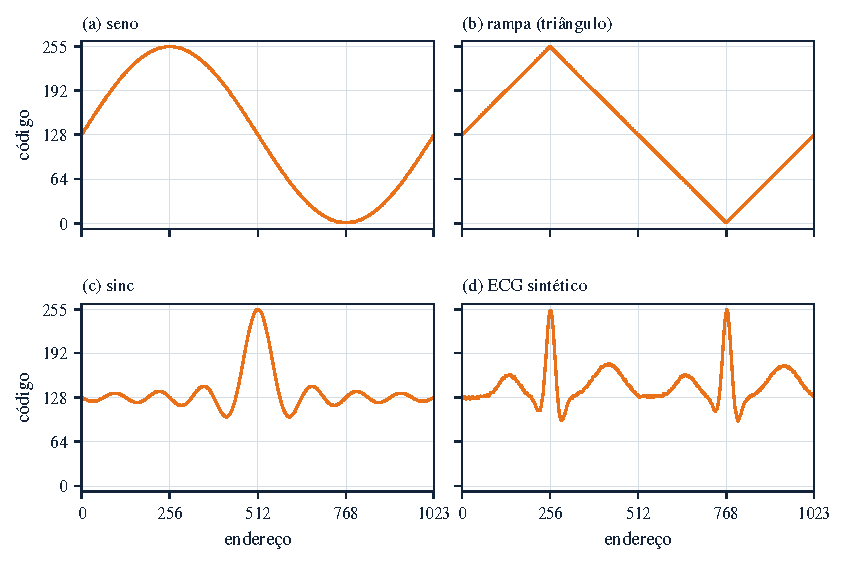
\includegraphics[width=\textwidth]{./figuras/luts}
	\legend{Fonte~---~Autoria própria.}
\end{figure}

As memórias registram o endereço e a saída, de modo que a amostra sai dois clocks depois do endereço. Após o multiplexador, a amostra passa por um registrador de saída (\cod{output\_register}), que no \eng{reset} assume o código 128, o zero do sinal. Esse registrador foi colocado nos registradores de entrada e saída do \ac{fpga}, junto aos pinos, para que os 8~bits mudem na mesma borda. Isso é importante porque o DAC0800 não tem registrador de entrada: bits que mudassem em instantes diferentes produziriam códigos intermediários na saída. O núcleo \cod{dds\_core} reúne o acumulador de fase, as tabelas e o registrador de saída; da fase até o pino do \ac{dac}, a latência é de três clocks.

\subsection{Controle pelo computador}\label{sec:controle}

O protocolo usa um registrador de instrução virtual de 2~bits e um registrador de dados de 18~bits, deslocado com o \ac{lsb} primeiro, conforme a Tabela~\ref{tab:protocolo}.

\begin{table}
	\caption{Instruções do protocolo de controle.}
	\label{tab:protocolo}
	\begin{tabular}{c l l}\toprule
		IR & Instrução & Conteúdo do DR (18~bits)\\\midrule
		\cod{00} & nenhuma (\eng{bypass}) & ---\\
		\cod{01} & frequência & frequência em hertz\\
		\cod{10} & forma de onda & \cod{sel} nos 2~bits menos significativos\\
		\cod{11} & escrita na tabela arbitrária & endereço (bits 17 a 8) e dado (bits 7 a 0)\\\bottomrule
	\end{tabular}
	\legend{Fonte~---~Autoria própria.}
\end{table}

O controle foi dividido em três blocos, um para cada domínio de clock e para a travessia entre eles:
\begin{description}
	\item[\cod{vjtag\_dr}] --- no domínio do \cod{tck}, desloca o registrador de dados durante o Shift-DR. No Update-DR, guarda a instrução e o valor deslocado e inverte o nível do sinal \cod{cmd\_toggle}, avisando que há um comando novo. No Capture-DR, carrega no registrador o último valor escrito com a mesma instrução, o que permite ler a configuração pelo \ac{jtag} para depuração. Na instrução \cod{00}, a saída \cod{tdo} vem de um registrador de \eng{bypass} de 1~bit;
	\item[\cod{cmd\_sync}] --- passa o comando para o domínio de 10~MHz pela técnica do \eng{toggle} descrita na Seção~\ref{sec:cdc}: apenas \cod{cmd\_toggle} passa por um sincronizador de três \eng{flip-flops}; quando sua mudança é detectada, os 20~bits do comando já estão estáveis e são copiados, com um pulso de um clock em \cod{dst\_valid}. A técnica exige que dois comandos estejam separados por mais de quatro ciclos de 10~MHz (0,4~\(\mu\)s). Um deslocamento de 18~bits leva mais de 22 ciclos de \cod{tck}, ou 3,7~\(\mu\)s a 6~MHz, frequência máxima do USB-Blaster, de forma que o requisito é sempre atendido;
	\item[\cod{control\_registers}] --- no domínio de 10~MHz, decodifica cada comando e atualiza os registradores de frequência e de forma de onda, ou gera um pulso de um clock na porta de escrita da \ac{ram}. Após o \eng{reset}, os registradores assumem 1~kHz e seno, de modo que a placa gera um sinal sem depender do computador.
\end{description}

Os três blocos foram agrupados na entidade \cod{jtag\_control}, que contém toda a lógica do controle mas não o \ac{ip} do Virtual \ac{jtag}. O \ac{ip} e o \cod{jtag\_control} são instanciados juntos em \cod{jtag\_interface}. Essa separação permite simular o controle completo, com o \eng{testbench} fazendo o papel do \ac{ip}, cujo modelo de simulação não gera sinais.

\subsection{Clock, reset e pinagem}

O \ac{pll} gera o clock de 10~MHz dividindo por cinco o oscilador de 50~MHz. O \eng{reset} do sistema vem do botão KEY[0] e da indicação de travamento do \ac{pll}, e passa por um sincronizador (\cod{reset\_sync}): entra em \eng{reset} de forma assíncrona, assim que o botão é pressionado, e sai em sincronia com o clock, três bordas depois de o botão ser solto. Assim, todos os registradores saem do \eng{reset} na mesma borda.

A Tabela~\ref{tab:pinos} mostra a pinagem, a mesma do código legado (Seção~\ref{sec:legado}), e a Figura~\ref{fig:pin_planner} mostra essas atribuições no Pin Planner do Quartus. O barramento do \ac{dac} usa os pinos 3 a 10 do conector de expansão, e o pino 1 é mantido em nível baixo como referência de terra no cabo. O pino 2 leva o clock de 10~MHz invertido, gerado pela entidade \cod{dac\_clock} com um registrador de saída de taxa dupla (\cod{altddio\_out}), o que evita passar o clock pela lógica. A borda de subida desse clock ocorre 50~ns depois da mudança dos bits, no meio da amostra. O DAC0800 não usa clock, mas o pino permite ligar um \ac{dac} com registrador de entrada e serve de gatilho para o osciloscópio. Dois \eng{LEDs} indicam o travamento do \ac{pll} e a chegada de cada comando do computador. A Tabela~\ref{tab:barramento} mostra o caminho de cada bit até o \acs{dac}: do pino do \acs{fpga} ao conector de expansão JP5 da DE2-115, dele ao conector J1 da placa analógica e, por fim, ao pino do DAC0800. A Figura~\ref{fig:jp5} mostra a disposição do JP5: os pinos ímpares ficam em uma fileira e os pares na outra, e o pino \(n\) corresponde ao GPIO[\(n - 1\)]. O fabricante numera as entradas do DAC0800 do bit mais significativo para o menos significativo, de B1 a B8, e por isso o bit 0 do \acs{fpga} chega à entrada B8, e o bit 7, à B1.

\begin{table}
	\caption{Pinagem do \acs{fpga} na placa DE2-115.}
	\label{tab:pinos}
	\begin{tabular}{l l l l}\toprule
		Porta & Pino do \acs{fpga} & Sinal na placa & Padrão de E/S e corrente\\\midrule
		\cod{clk\_50} & PIN\_Y2 & CLOCK\_50 & LVTTL 3,3~V\\
		\cod{rst\_n} & PIN\_M23 & botão KEY[0] & LVTTL 3,3~V\\
		\cod{dac(0)} & PIN\_AB21 & GPIO[2] & LVTTL 3,3~V, 8~mA\\
		\cod{dac(1)} & PIN\_Y17 & GPIO[3] & LVTTL 3,3~V, 8~mA\\
		\cod{dac(2)} & PIN\_AC21 & GPIO[4] & LVTTL 3,3~V, 8~mA\\
		\cod{dac(3)} & PIN\_Y16 & GPIO[5] & LVTTL 3,3~V, 8~mA\\
		\cod{dac(4)} & PIN\_AD21 & GPIO[6] & LVTTL 3,3~V, 8~mA\\
		\cod{dac(5)} & PIN\_AE16 & GPIO[7] & LVTTL 3,3~V, 8~mA\\
		\cod{dac(6)} & PIN\_AD15 & GPIO[8] & LVTTL 3,3~V, 8~mA\\
		\cod{dac(7)} & PIN\_AE15 & GPIO[9] & LVTTL 3,3~V, 8~mA\\
		\cod{dac\_clk} & PIN\_AC15 & GPIO[1] & LVTTL 3,3~V, 8~mA\\
		\cod{dac\_gnd} & PIN\_AB22 & GPIO[0] & LVTTL 3,3~V, 8~mA\\
		\cod{led\_locked} & PIN\_E21 & \eng{LED} LEDG[0] & 2,5~V, 8~mA\\
		\cod{led\_cmd} & PIN\_E22 & \eng{LED} LEDG[1] & 2,5~V, 8~mA\\\bottomrule
	\end{tabular}
	\legend{Fonte~---~Autoria própria.}
\end{table}

\begin{table}
	\caption{Ligação do barramento, do \acs{fpga} ao DAC0800.}
	\label{tab:barramento}
	\begin{tabular}{l l l c c c}\toprule
		Bit & Porta & Pino do \acs{fpga} & Conector JP5 & Conector J1 & Pino do DAC0800\\\midrule
		0 (\acs{lsb}) & \cod{dac(0)} & PIN\_AB21 & 3 & 1 & 12 (B8)\\
		1 & \cod{dac(1)} & PIN\_Y17 & 4 & 2 & 11 (B7)\\
		2 & \cod{dac(2)} & PIN\_AC21 & 5 & 3 & 10 (B6)\\
		3 & \cod{dac(3)} & PIN\_Y16 & 6 & 4 & 9 (B5)\\
		4 & \cod{dac(4)} & PIN\_AD21 & 7 & 5 & 8 (B4)\\
		5 & \cod{dac(5)} & PIN\_AE16 & 8 & 6 & 7 (B3)\\
		6 & \cod{dac(6)} & PIN\_AD15 & 9 & 7 & 6 (B2)\\
		7 (\acs{msb}) & \cod{dac(7)} & PIN\_AE15 & 10 & 8 & 5 (B1)\\
		--- & \cod{dac\_clk} & PIN\_AC15 & 2 & --- & ---\\
		--- & \cod{dac\_gnd} & PIN\_AB22 & 1 & --- & ---\\\bottomrule
	\end{tabular}
	\legend{Fonte~---~Autoria própria.}
\end{table}

\begin{figure}
	\caption{Atribuição dos pinos no Pin Planner do Quartus.}
	\label{fig:pin_planner}
	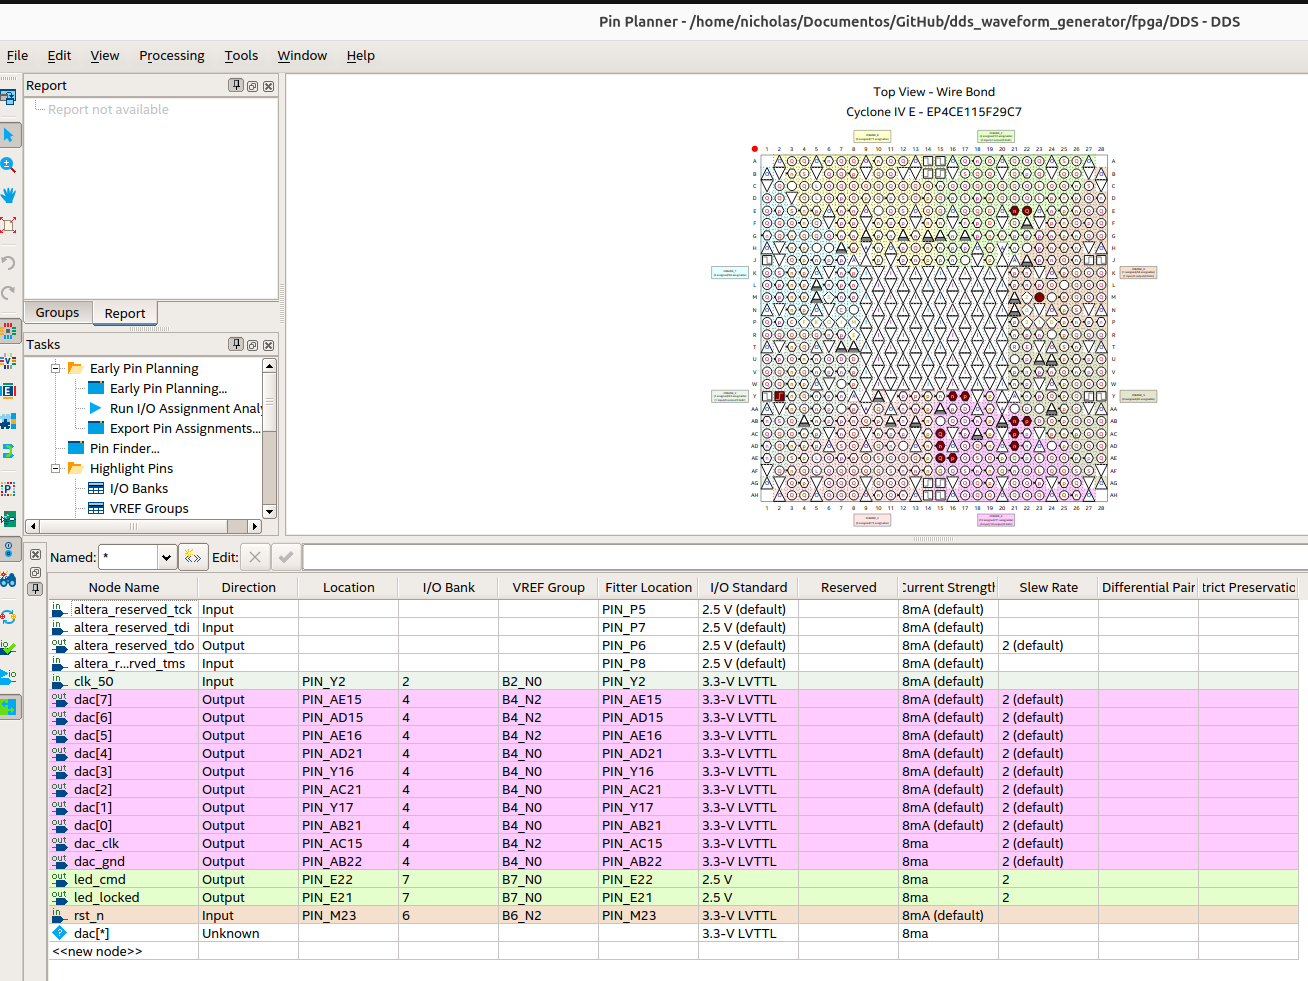
\includegraphics[width=\textwidth]{./figuras/pin_planner}
	\legend{Fonte~---~Autoria própria.}
\end{figure}

\begin{figure}
	\caption{Conector de expansão JP5 da DE2-115, com o pino do \acs{fpga} ligado a cada posição.}
	\label{fig:jp5}
	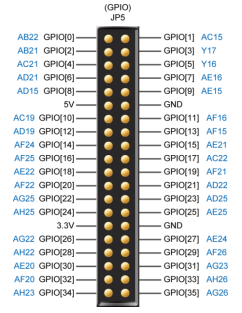
\includegraphics[width=0.4\textwidth]{./figuras/jp5_gpio}
	\legend{Fonte~---~Terasic Technologies \cite{terasic2010}.}
\end{figure}


As restrições de tempo foram descritas em um arquivo \ac{sdc}: o clock de 50~MHz e os clocks derivados do \ac{pll}; o clock do \ac{jtag} como assíncrono em relação aos demais, já que a travessia é tratada pelo \cod{cmd\_sync}; e caminhos sem requisito de tempo para o botão, os \eng{LEDs}, o barramento do \ac{dac}, que não usa clock, e o próprio clock do \ac{dac}, cuja relação com os dados é fixada pelos registradores junto aos pinos.

\section{Verificação por simulação}

Cada bloco do projeto digital tem um \eng{testbench} auto-verificável, escrito em \ac{vhdl}-2008 e executado no simulador GHDL \cite{ghdl2025}. Os blocos gerados pela Intel são simulados com os modelos da biblioteca \cod{altera\_mf}, distribuída com o Quartus. Cada \eng{testbench} compara a saída do bloco, ciclo a ciclo, com um modelo de referência escrito no próprio \eng{testbench}, conta os erros e termina com a mensagem \enquote{OK} apenas se não houver nenhum. Para o núcleo \ac{dds}, por exemplo, o modelo calcula a fase pela Equação~(\ref{eq:acumulador}), o endereço pelo truncamento e a amostra esperada pela tabela correspondente, considerando a latência de três clocks.

Os blocos do controle são verificados com um modelo de comportamento do Virtual \ac{jtag}: procedimentos que geram o \cod{tck}, a instrução e a sequência Capture-DR, Shift-DR e Update-DR, como o \ac{ip} faria a cada comando do \cod{quartus\_stp}. A Tabela~\ref{tab:testbenches} lista os 16 \eng{testbenches} e o que cada um confere. Um \eng{script} compila os fontes e executa todos eles em sequência. Para as figuras deste texto, os \eng{testbenches} são executados gravando os sinais de interesse em arquivos \ac{vcd}, que um \eng{script} em Python lê e desenha.

\begin{table}
	\caption{\eng{Testbenches} do projeto digital.}
	\label{tab:testbenches}
	\begin{tabular}{l p{0.62\textwidth}}\toprule
		\eng{Testbench} & O que é conferido\\\midrule
		\cod{tb\_frequency\_translator} & as \(2^{18}\) entradas: \ac{ftw} conforme a Equação~(\ref{eq:ftw}) e erro menor que 1~\ac{lsb}\\
		\cod{tb\_word\_adder} & soma com estouro, casos de borda e 10\,000 pares aleatórios\\
		\cod{tb\_phase\_register} & carga apenas na borda de subida e \eng{reset} assíncrono\\
		\cod{tb\_truncator} & endereço igual aos 10~bits mais significativos da fase\\
		\cod{tb\_phase\_accumulator} & endereço ciclo a ciclo, trocas de frequência sem salto de fase\\
		\cod{tb\_out\_mux} & seleção para cada código de \cod{sel}\\
		\cod{tb\_LUT} & os 1024 endereços das três \acp{rom} e da \ac{ram}, escrita durante a leitura\\
		\cod{tb\_output\_register} & código 128 no \eng{reset} e carga na borda\\
		\cod{tb\_dds\_core} & cada amostra contra o modelo, nas quatro formas e com trocas em operação\\
		\cod{tb\_reset\_sync} & entrada imediata e saída na terceira borda\\
		\cod{tb\_vjtag\_dr} & deslocamento, comando no Update-DR, leitura no Capture-DR e \eng{bypass}\\
		\cod{tb\_cmd\_sync} & 300 comandos de 6~MHz para 10~MHz, todos entregues uma vez e em ordem\\
		\cod{tb\_control\_registers} & valores após o \eng{reset}, decodificação e pulso de escrita\\
		\cod{tb\_jtag\_control} & do registrador de dados do \ac{jtag} até os registradores de configuração\\
		\cod{tb\_system} & do comando do computador até a amostra do \ac{dac}, incluindo o envio de uma tabela\\
		\cod{tb\_DDS} & entidade do topo com o \ac{pll}: clocks, \eng{LEDs}, seno de 1~kHz e \eng{reset}\\\bottomrule
	\end{tabular}
	\legend{Fonte~---~Autoria própria.}
\end{table}

\section{Interface com o usuário}

A interface gráfica foi escrita em Python 3.12, com a biblioteca Tkinter, e usa apenas a biblioteca padrão da linguagem. Ela mantém aberto um processo do \cod{quartus\_stp} e envia a ele comandos Tcl: trava o acesso ao \ac{jtag}, desloca a instrução uma vez e o registrador de dados uma vez para cada valor, e libera o acesso. Uma \eng{thread} separada executa os comandos em ordem e devolve os resultados por uma fila de eventos, de modo que a janela não trava durante o envio de uma tabela, que exige 1024 deslocamentos.

A interface permite escolher a frequência, mostrando a palavra de sintonia calculada pela Equação~(\ref{eq:ftw}), e a forma de onda; carregar a tabela arbitrária de um arquivo \ac{mif} ou de um arquivo de texto com 1024 valores, ou gerá-la a partir de formas prontas; visualizar a tabela antes do envio; e acompanhar as mensagens do \cod{quartus\_stp} em um console. A Figura~\ref{fig:interface} mostra a interface: no alto, a conexão \acs{jtag} e a carga da tabela arbitrária; à esquerda, a frequência, com a palavra de sintonia correspondente, a forma de onda e os parâmetros do sistema; ao centro, o gráfico da tabela arbitrária; e, abaixo, o console.

Para dispensar o terminal, a interface foi empacotada com o PyInstaller em um executável único, que já contém o Python, o Tkinter, o ícone e as tabelas \ac{mif}, e um atalho no menu de aplicativos a abre com dois cliques. Ela depende apenas do Quartus instalado, de onde vem o \cod{quartus\_stp}.

\begin{figure}
	\caption{Interface gráfica de controle do gerador.}
	\label{fig:interface}
	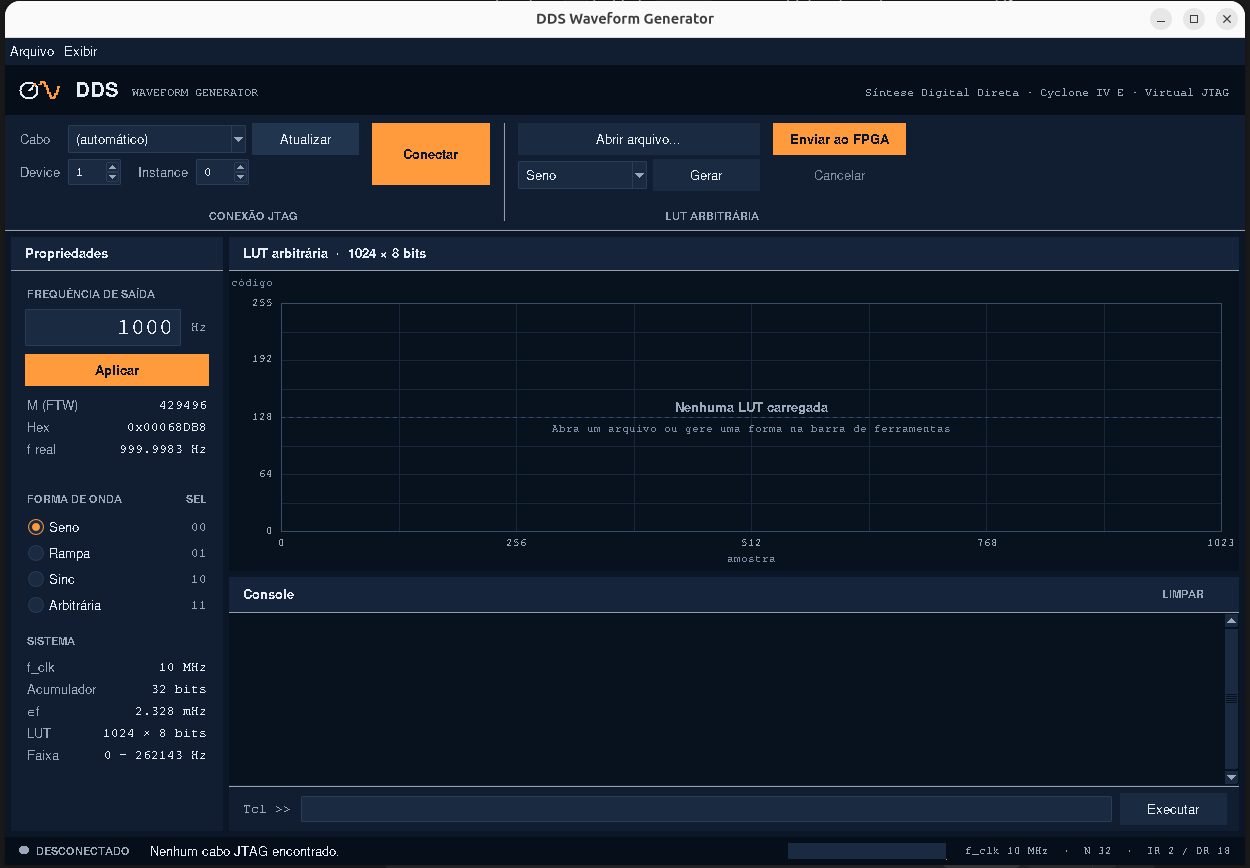
\includegraphics[width=\textwidth]{./figuras/interface}
	\legend{Fonte~---~Autoria própria.}
\end{figure}

\section{Placa analógica}

A placa analógica recebe os 8~bits pelo conector J1 e é alimentada com \(\pm15\)~V, para os amplificadores operacionais e o \ac{dac}, e +10~V, para a referência do \ac{dac}. O circuito tem cinco blocos, ligados conforme a Figura~\ref{fig:sistema}. Os valores a seguir são os da simulação do circuito, que segue a mesma topologia da placa.

O DAC0800 tem a referência de 10~V aplicada através de um resistor de 5~k\(\Omega\), o que, pela Equação~(\ref{eq:dac0800}), fixa \(I_{REF} = 2\)~mA e \(I_{FS} \approx 1{,}992\)~mA. Com o pino de limiar lógico no terra, o limiar das entradas é de 1,4~V, compatível com a lógica de 3,3~V do \ac{fpga}. Na placa, o pino DB7 do conector J1, que recebe o \ac{msb} da amostra, é ligado à entrada B1 do conversor, que é o seu \ac{msb}.

As duas saídas de corrente alimentam um amplificador de diferenças com quatro resistores de 1~k\(\Omega\), cuja saída é
\begin{equation}\label{eq:vdif}
	V_{dif} = \left(I_{OUT} - \overline{I_{OUT}}\right) \cdot 1~\mathrm{k}\Omega,
\end{equation}
que vai de \(-1{,}99\)~V, no código 0, a \(+1{,}99\)~V, no código 255. Em seguida, um filtro Sallen-Key de ganho unitário, com \(R_1 = R_2 = 48~\Omega\) e \(C_1 = C_2 = 3{,}3\)~nF, tem, pela Equação~(\ref{eq:sallen_key}), \(f_0 \approx 1{,}00\)~MHz e \(Q = 0{,}5\). A resposta em frequência, mostrada na Figura~\ref{fig:filtro}, tem atenuação de 3~dB em 647~kHz, perda de 0,6~dB na frequência máxima do gerador e atenuação de cerca de 40~dB em \(f_{clk}\), onde surgem as primeiras imagens.

\begin{figure}
	\caption{Resposta em frequência do filtro de reconstrução.}
	\label{fig:filtro}
	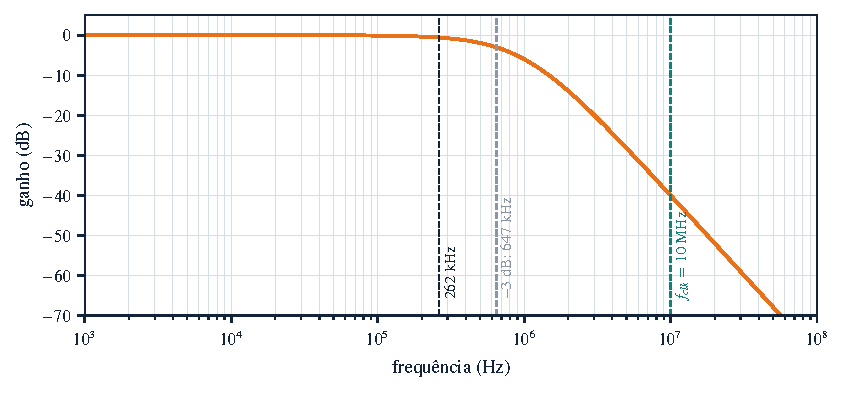
\includegraphics[width=\textwidth]{./figuras/filtro}
	\legend{Fonte~---~Autoria própria.}
\end{figure}

O ganho é ajustado por um amplificador inversor com um potenciômetro de 10~k\(\Omega\) (VR1). Por fim, um seguidor de tensão entrega o sinal ao conector de saída J7. Os quatro amplificadores são as quatro seções de um TL074.

A placa foi desenhada com mais um estágio depois do seguidor: um par complementar BC847 e BC857, polarizado por dois diodos LL4148 em classe AB, para aumentar a corrente de saída. Esse estágio foi retirado por apresentar distorção e resultados inesperados nos ensaios, e a saída passou a ser tomada diretamente do seguidor.

A placa foi projetada no Altium Designer e fabricada em duas faces. A Figura~\ref{fig:pcb_esquematico} mostra o esquemático, a Figura~\ref{fig:pcb_layout}, o layout das trilhas, e a Figura~\ref{fig:placa}, a vista tridimensional e a placa montada. O esquemático e o layout ainda incluem o estágio classe AB (Q1, Q2, D1, D2, R11 e R12), que foi retirado da montagem. O circuito, sem o estágio classe AB, foi simulado no LTspice com um macromodelo comportamental do DAC0800, escrito pelo autor a partir das características típicas da folha de dados \cite{ti2013,seifert2026spice} e descrito no Apêndice~\ref{ap:dac0800}: referência, divisão da corrente entre as saídas, limiar lógico, tempo de comutação de 70~ns e limites de conformidade das saídas. Os estímulos das entradas digitais são fontes lineares por partes geradas a partir da simulação do \ac{vhdl}, para uma senoide de 1~kHz. A Figura~\ref{fig:ltspice} mostra o esquemático simulado, com os nós cujas tensões são analisadas no Capítulo~\ref{cap:resultados}.

\begin{figure}
	\caption{Esquemático da simulação da placa analógica no LTspice: fontes dos estímulos (U7), DAC0800 (U1), conversor corrente-tensão (U2), estágio de ganho (U3), filtro de reconstrução (U4) e \eng{buffer} (U5).}
	\label{fig:ltspice}
	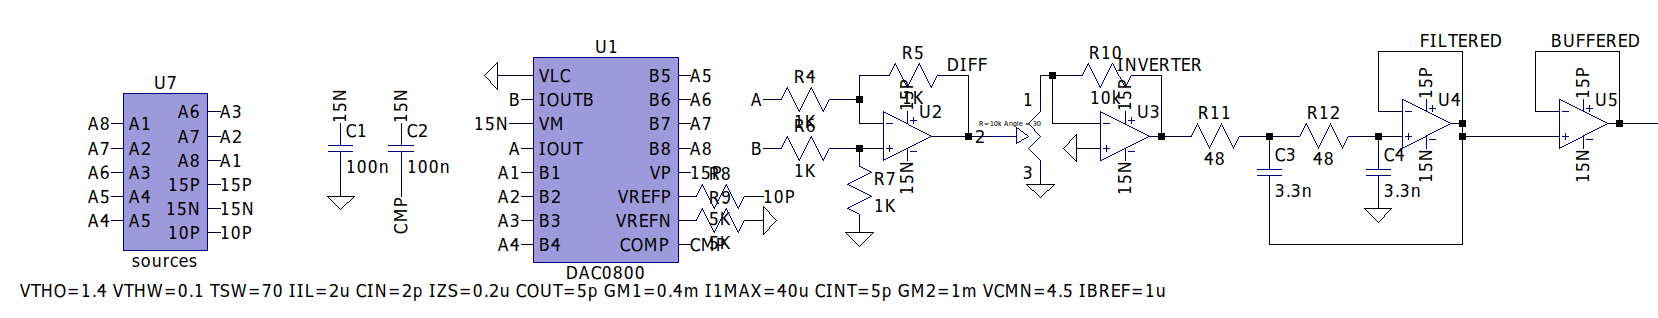
\includegraphics[width=\textwidth]{./figuras/ltspice_esquematico}
	\legend{Fonte~---~Autoria própria.}
\end{figure}


\begin{figure}
	\caption{Esquemático da placa analógica.}
	\label{fig:pcb_esquematico}
	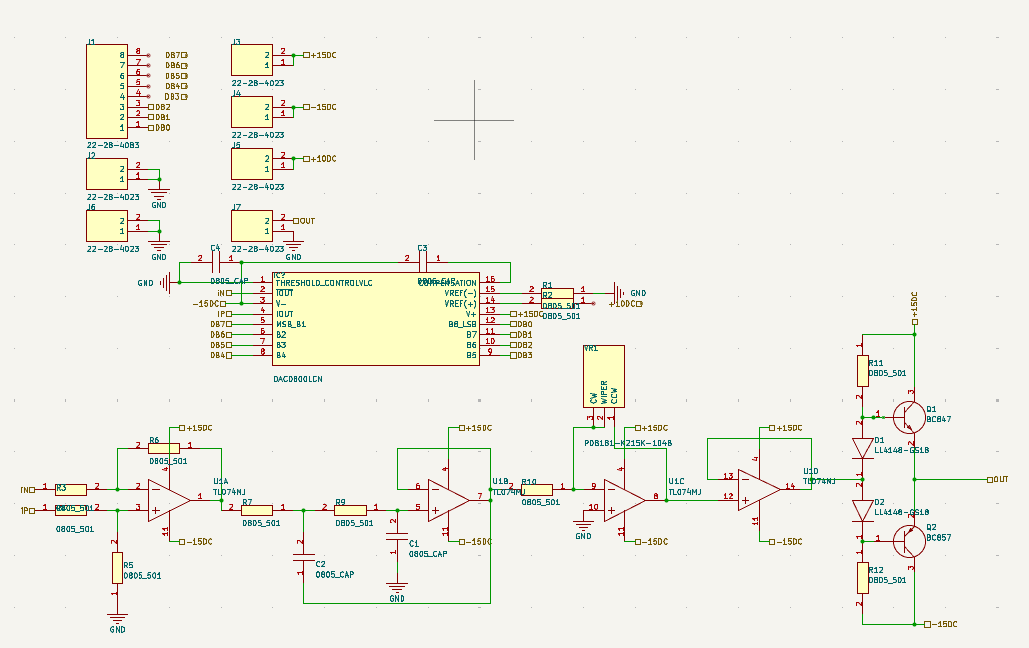
\includegraphics[width=\textwidth]{./figuras/pcb_esquematico}
	\legend{Fonte~---~Autoria própria.}
\end{figure}

\begin{figure}
	\caption{Layout da placa analógica: trilhas na face superior, em vermelho, e na inferior, em azul.}
	\label{fig:pcb_layout}
	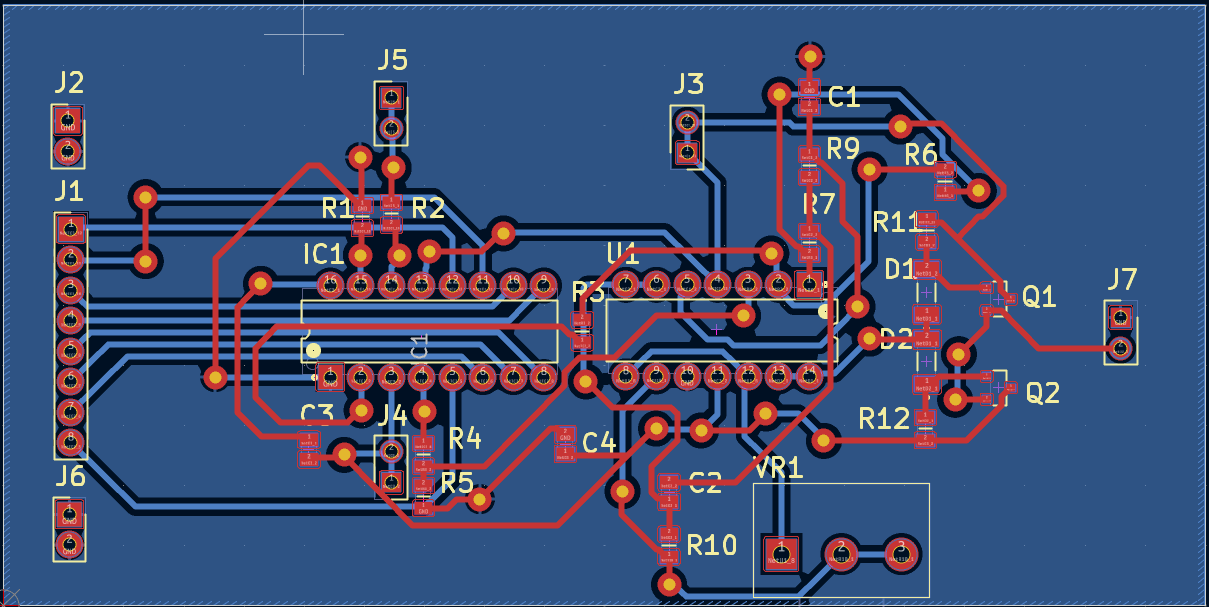
\includegraphics[width=\textwidth]{./figuras/pcb_layout}
	\legend{Fonte~---~Autoria própria.}
\end{figure}

\begin{figure}
	\caption{Placa analógica: (a) vista tridimensional; (b) placa montada, com o DAC0800 (IC1), o TL074 (U1) e o potenciômetro de ganho (VR1).}
	\label{fig:placa}
	\begin{minipage}[b]{0.6\textwidth}
		\centering
		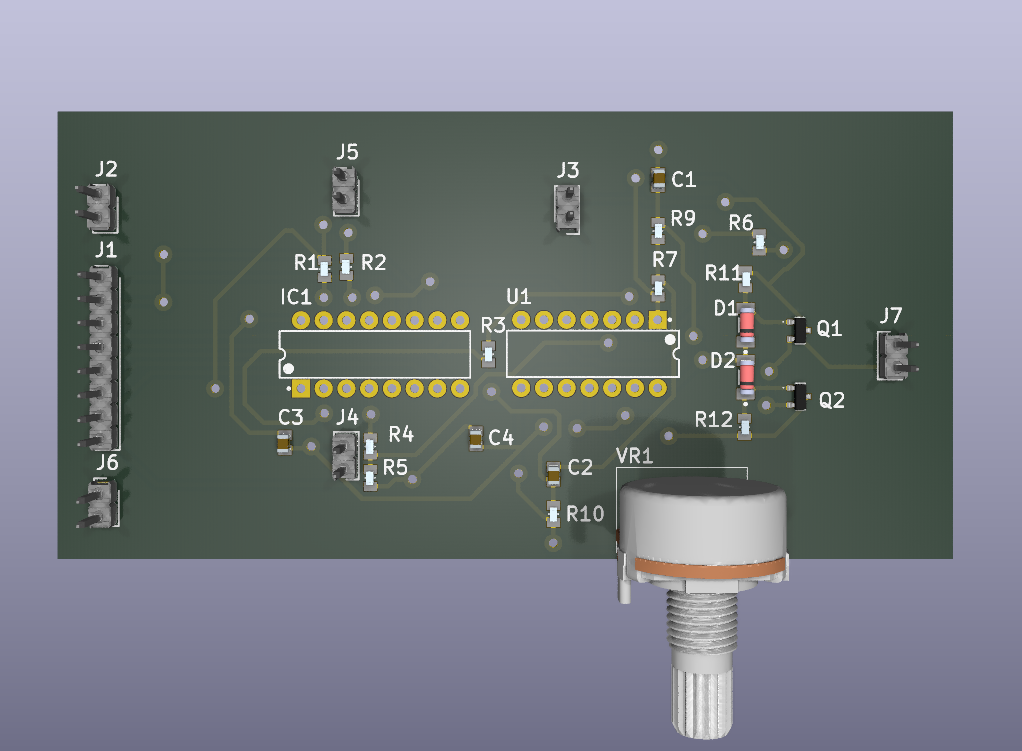
\includegraphics[height=6.4cm]{./figuras/pcb_3d}\\[2pt]
		{\smallfont (a)}
	\end{minipage}%
	\hfill
	\begin{minipage}[b]{0.36\textwidth}
		\centering
		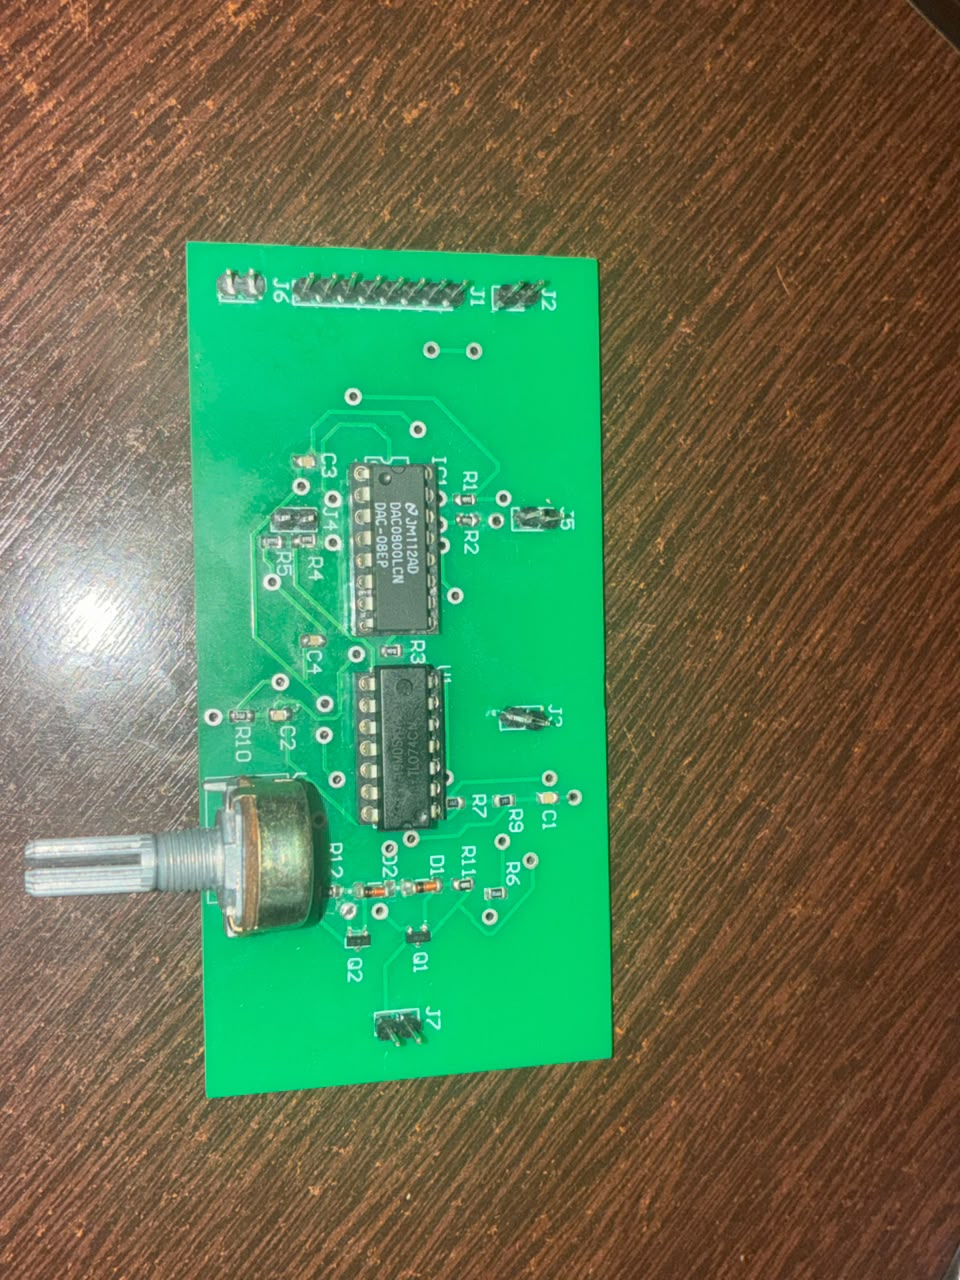
\includegraphics[height=6.4cm]{./figuras/placa}\\[2pt]
		{\smallfont (b)}
	\end{minipage}
	\legend{Fonte~---~Autoria própria.}
\end{figure}
